\section{Introduction}\label{sec:introduction}
The splitting-off operation in undirected graphs is a simple yet powerful operation in graph theory.  
It is a reduction operation that detaches all edges incident to a given vertex and adds new edges between the neighbors of that vertex while preserving their degrees. 
%and edge-connectivity. 
Equivalently, it enables a vertex to exit the network by informing its neighbors  
how to reconfigure the lost links 
among themselves in order to preserve their degrees.
%edge-connectivity (as well as degrees). 
Lov\'{a}sz \cite{Lov74, Lovasz-problems-book} introduced the splitting-off operation and showed the existence of the operation to preserve global edge-connectivity under certain conditions. Mader \cite{Mad78} showed the existence of the splitting-off operation to preserve local edge-connectivity (i.e., all pairwise edge-connectivities) under certain conditions. 
Both Lov\'{a}sz's and Mader's results also admit strongly polynomial-time algorithms \cite{Frank-book, nagamochi_ibaraki_2008_book, Gab94}. 
%The inductive nature of the splitting-off operation leads to far ranging applications in graph theory, algorithms, and optimization. It enables fundamental graph theoretical results such as constructive characterization of $k$-edge-connected graphs \cite{??}. 
Owing to the inductive nature of the splitting-off operation, Lov\'{a}sz's and Mader's results have enabled fundamental results in graph theory as well as efficient algorithms and min-max relations for numerous graph optimization problems. 
In fact, Mader \cite{Mad78} illustrated the power of his local edge-connectivity preserving splitting-off result by deriving Nash-Williams' strong orientation theorem \cite{NW60} (also see Frank's exposition of this derivation \cite{Frank93:Applications-of-submod-functions}).  
%\shubhang{(side) note: \cite{Gab94} gives an efficient implementation of Frank's proof of the Strong Orientation Theorem.}). 
%In particular, it has been used 
Subsequently, the splitting-off operation 
has been used 
to give a constructive characterization of $k$-edge-connected graphs \cite{Frank-book} 
 and 
to address problems in edge-connectivity augmentation \cite{Fra92, Fra94, JFJ95, Frank-book, nagamochi_ibaraki_2008_book}, graph orientation \cite{FK02, Kiraly-Lau}, minimum cuts enumeration \cite{NNI97, HW96, Goe01}, network design \cite{Lov76, GB93, Jor03, CS08, CFLY11}, tree packing \cite{BHTP03, Kri03, JMS03, Lau07}, congruency-constrained cuts \cite{NZ20}, and approximation algorithms for TSP \cite{GB93, BN23}. 
Designing fast algorithms for global/local edge-connectivity preserving splitting-off remains an active area of research (e.g., see recent works \cite{LY13, CLP22-soda, CLP22-stoc, CHLP23}) due to these far-reaching applications. 
%We refer the reader to the textbooks by Frank \cite{Frank-book} and by Nagamochi and Ibaraki \cite{nagamochi_ibaraki_2008_book} for efficient algorithms to compute global/local edge-connectivity preserving splitting-off and some of their applications. 
In this work, we introduce a splitting-off operation in \emph{hypergraphs}, show the existence of local-connectivity preserving splitting-off operation, design a strongly polynomial-time algorithm to compute it in weighted hypergraphs, and illustrate its usefulness by showing two applications. 

\paragraph{Hypergraphs.}
Hypergraphs offer a richer and more accurate model than graphs for several applications. 
Consequently, hypergraphs have found applications in several modern areas (e.g., see \cite{VeldtBK22,Schlagetal23,LiM17, Ornes21}) and these applications have, in turn, driven exciting recent progress in algorithms for hypergraph optimization problems \cite{KK15, GKP17, CXY19-j, CX18, CC22, CKN20, SY19, BST19, KKTY21-FOCS, KKTY21-STOC, Lee22, JLS22, Quanrud22, GLSTW22, CC23, AGL23, FPZ23}. 
A hypergraph $G=(V, E)$ consists of a finite set $V$ of vertices and a set $E$ of hyperedges, where every hyperedge $e\in E$ is a subset of $V$. We will denote a hypergraph $G=(V, E)$ with hyperedge weights $w: E\rightarrow \Z_+$ by the tuple $(G, w)$ and use $G_w$ to denote the unweighted multi-hypergraph over vertex set $V$ containing $w(e)$ copies of every hyperedge $e\in E$.  
Throughout this work, we will be interested only in hypergraphs with positive integral weights and for algorithmic problems where the input/output is a hypergraph, we will require that the weights are represented in binary. 
If all hyperedges have size at most $2$, then the hyperedges are known as edges and we call such a hypergraph as a graph. 
We emphasize a subtle but important distinction between hypergraphs and graphs: the number of hyperedges in a hypergraph could be exponential in the number of vertices. This is in sharp contrast to graphs where the number of edges is at most the square of the number of vertices. Consequently, in hypergraph network design problems where the goal is to construct a hypergraph with certain properties,  
one needs to be mindful of the number of hyperedges in the hypergraph returned by the algorithm. %We mention that recent 
Recent works in hypergraph algorithms literature have 
%addressed this precise 
focused on this 
issue in the context of cut/spectral sparsification of hypergraphs \cite{KK15, CX18, SY19, BST19, CKN20, KKTY21-FOCS, KKTY21-STOC, Lee22, JLS22, Quanrud22}. 


\iffalse
A hypergraph $H=(V, E)$ consists of a finite set $V$ of vertices and a set $E$ of hyperedges, where every hyperedge $e\in E$ is a subset of $V$. We will denote a hypergraph $H=(V, E)$ with hyperedge weights $w: E\rightarrow \Z_+$ by the tuple $(H, w)$ and use $H_w$ to denote the unweighted multi-hypergraph over vertex set $V$ containing $w(e)$ copies of every hyperedge $e\in E$.  
Throughout this work, we will be interested only in hypergraphs with positive integral weights and for algorithmic problems where the input/output is a hypergraph, we will require that the weights are represented in binary. 
If all hyperedges have size at most $2$, then the hyperedges are known as edges and we call such a hypergraph as a graph. 
Hypergraphs offer a richer and more accurate model than graphs for several applications. 
Consequently, hypergraphs have found applications in several modern areas (e.g., see \cite{VeldtBK22,Schlagetal23,LiM17, Ornes21}) and these applications have, in turn, driven exciting recent progress in algorithms for hypergraph optimization problems \cite{KK15, GKP17, CXY19-j, CX18, CC22, CKN20, SY19, BST19, KKTY21-FOCS, KKTY21-STOC, Lee22, JLS22, Quanrud22}. 
We emphasize a subtle but important distinction between hypergraphs and graphs: the number of hyperedges in a hypergraph could be 
%We note that the number of hyperedges in a hypergraph could be 
exponential in the number of vertices. This is in sharp contrast to graphs where the number of edges is at most the square of the number of vertices. Consequently, in hypergraph network design problems where the goal is to construct a hypergraph with certain properties,  
one needs to be mindful of the number of hyperedges in the hypergraph returned by the algorithm. 
\fi

\iffalse
Recent works have explored this issue in the context of hypergraph sparsifiers \cite{KK15, CX18, SY19, BST19, CKN20, KKTY21-FOCS, KKTY21-STOC, Lee22, JLS22, Quanrud22}  
and shown that every hypergraph (possibly with exponential number of hyperedges) admits a cut/coverage/spectral sparsifier
in which the number of hyperedges is near-linear in the number of vertices and such a sparsifier can be constructed in time near-linear in the size of the input hypergraph. 
\knote{Perhaps, this discussion about exponential number of hyperedges is better done after defining splitting-off.} 
\fi

\paragraph{Notation.} Let $(G=(V, E), w: E\rightarrow \Z_+)$ be a hypergraph. 
For $X\subseteq V$, let $\delta_G(X)\coloneqq \{e\in E: e\cap X\neq \emptyset, e\setminus X\neq \emptyset\}$.  
We define the cut function $d_{(G, w)}: 2^V\rightarrow \Z_{\ge 0}$ by $d_{(G, w)}(X) \coloneqq \sum_{e\in \delta_G(X)}w(e)$ for every $X\subseteq V$. 
For a vertex $v\in V$, we use $d_{(G,w)}(v)$ to denote $d_{(G,w)}(\{v\})$. 
We define the degree of a vertex $v$ to be the sum of the weights of hyperedges containing $v$---we note that the degree of a vertex is not necessarily equal to $d_{(G, w)}(v)$ since we could have $\{v\}$ itself as a hyperedge (i.e., a singleton hyperedge that contains only the vertex $v$). 
For distinct vertices $u, v\in V$, let $\lambda_{(G, w)}(u, v)\coloneqq \min\{d_{(G, w)}(X): u\in X\subseteq V\setminus \{v\}\}$ -- i.e., $\lambda_{(G, w)}(u, v)$ is the value of a minimum $\{u, v\}$-cut in the hypergraph. If all hyperedge weights are unit, then we drop $w$ from the subscript and simply use $d_G$ and $\lambda_G$. 

\paragraph{Hypergraph Splitting-off.} 
%A notion of hypergraph splitting-off motivated by hypergraph connectivity augmentation applications has been studied in the literature before \cite{BJ99, Cosh-thesis, BK12}. These works have explored splitting-off a vertex $s$ from a hypergraph under the assumption that all hyperedges incident to the vertex $s$ are in fact edges. In contrast, we are interested in splitting-off at a vertex $s$ from a hypergraph without such an assumption (i.e., the vertex $s$ could have arbitrary-sized hyperedges incident to it) \knote{This may not be informative for a reader unfamiliar with the splitting-off operation.}. 
We now introduce our definition of splitting-off in hypergraphs. 
To compare and contrast our definition of splitting-off for hypergraphs with the classical definition of splitting-off for graphs, we include both our definition and the classical definition and distinguish them by identifying them as h-splitting-off and g-splitting-off. 
%(with the convention being that we add the prefix `h' for hypergraph related terminology and the prefix `g' for graph related terminology). 
In the definitions below, we encourage the reader to consider the input hypergraph $(G, w)$ to be a graph while considering g-splitting-off terminology and to be a hypergraph while considering h-splitting-off terminology. We encourage the reader to also assume unit weights during first read. See Figure \ref{figure:hypergraph-splitting-off-example-1} for an example. 

\begin{definition}\label{defn:splitting-off}
    Let $(G=(V, E), w: E\rightarrow \Z_+)$ be a hypergraph and $s\in V$. 
    \begin{enumerate}
            
        \item 
        In \emph{merge almost-disjoint hyperedges}, we pick a pair of hyperedges $e, f\in \delta_G(s)$ such that $e\cap f=\{s\}$, pick a positive integer $\alpha \in \Z_+$ such that $\alpha\le \min\{w(e), w(f)\}$, reduce the weights of hyperedges $e$ and $f$ by $\alpha$, and increase the weight of a hyperedge $g$ by $\alpha$. Here, 
        \begin{enumerate}
            \item if we choose $g\coloneqq e \cup f$, then the associated operation will be called as \emph{h-merge almost-disjoint hyperedges operation}.
            \item if we choose $g\coloneqq (e\cup f)\setminus \{s\}$, then the associated operation will be called as \emph{g-merge almost-disjoint hyperedges operation}.
        \end{enumerate}
        In the above, if $\alpha=w(e)$ (resp. if $\alpha = w(f)$), then we discard the hyperedge $e$ (resp. hyperedge $f$) from the hypergraph obtained after the operation; if the hyperedge $g\not\in E$, then we introduce $g$ as a new hyperedge with weight $w(g) := 0$ before performing the weight increase on the hyperedge $g$.
    
        \item 
        In \emph{trim hyperedge operation}, we pick a hyperedge $e\in \delta_G(s)$, pick a positive integer $\alpha \in \Z_+$,
        reduce the weight of the hyperedge $e$ and 
        increase the weight of the hyperedge $g\coloneqq e\setminus \{s\}$. Here, 
        \begin{enumerate}
            \item if we choose $\alpha \le w(e)$, reduce the weight of the hyperedge $e$ by $\alpha$,  and increase the weight of the hyperedge $g$ by $\alpha$, then the associated operation will be called as \emph{h-trim operation} (if $\alpha=w(e)$, then we discard $e$ from the hypergraph obtained after the operation; if $g\not\in E$, then we add $g$ as a new hyperedge with weight $w(g) := 0$ before performing the weight increase on the hyperedge $g$). 
            
            \item if we choose $\alpha \le w(e)/2$, reduce the weight of the hyperedge $e$ by $2\alpha$, and increase the weight of the hyperedge $g$ by $2\alpha$, then the associated operation will be called as \emph{g-trim operation} (if $\alpha=w(e)/2$, then we discard $e$ from the hypergraph obtained after the operation; if $g\not\in E$, then we add $g$ as a new hyperedge with weight $w(g) := 0$ before performing the weight increase on the hyperedge $g$).  
        \end{enumerate}

\item We say that a hypergraph $(H=(V, E_H), w_H: E_H\rightarrow \Z_+)$ is obtained by applying a 
        \begin{enumerate}
            \item \emph{h-splitting-off operation at $s$ from $(G, w)$} if $(H, w_H)$ is obtained from $(G, w)$ by either the h-merge almost-disjoint hyperedges operation or the h-trim hyperedge operation. 
            \item \emph{g-splitting-off operation at $s$ from $(G, w)$} if $(H, w_H)$ is obtained from $(G, w)$ by either the g-merge almost-disjoint hyperedges operation or the g-trim hyperedge operation. 
        \end{enumerate}

%\iffalse
\end{enumerate}
\end{definition}
Certain remarks regarding the definitions are in order. 
%h-splitting-off and g-splitting-off \emph{almost-disjoint} hyperedges operations ensure that the degree of every vertex $u\in V\setminus\{s\}$ is preserved. 
%However, if we allow the same operations for an arbitrary pair of hyperedges $e, f\in \delta_G(s)$, then degrees of vertices $u\in V\setminus \{s\}$ may not be preserved. 
%Similarly, both h-trimming and g-trimming operations preserve the degree of every vertex $u\in V\setminus \{s\}$. 
Firstly, the trim operation is valuable and unique to hypergraphs. It has been used in the hypergraph literature to obtain small-sized certificates for hypergraph connectivity \cite{CX18} and for certain notions of directed hypergraph connectivity \cite{Frank-book}. 
We note that the trim operation has limited value in graphs---trimming an edge leads to a singleton edge and singleton edges contribute only to the degree but not to the cut value of any set. 
%However, the trimming operation in graphs has limited value. 
Secondly, all operations mentioned above are degree preserving for vertices $u\in V\setminus \{s\}$: both h-trim and g-trim operations preserve degrees by definition; both h-merge and g-merge \emph{almost-disjoint} hyperedges operations preserve degrees due to the almost-disjoint property of the chosen hyperedges. 
Thirdly, all operations mentioned above 
%both h-merge operation and g-splitting-off operations 
\emph{do not} increase the %coverage/
cut values of subsets $X\subseteq V\setminus\{s\}$. Thus, the relevant goal with these operations is ensuring that the cut values do not decrease too much---i.e., preserving global/local connectivity. 
We will be interested in repeated application of h-splitting-off operations at a vertex from a given hypergraph to isolate that vertex while preserving global/local connectivity. We define these formally next. 
\begin{definition}
    Let $(G=(V, E), w: E\rightarrow \Z_+)$ be a hypergraph and $s\in V$. 
    \begin{enumerate}
    %\fi
        \item We say that a hypergraph $(G^*=(V, E^*), w^*: E^*\rightarrow \Z_+)$ is a 
        \begin{enumerate}
            \item \emph{complete h-splitting-off at $s$ from $(G, w)$} if $d_{(G^*, w^*)}(s) = 0$ and $(G^*, w^*)$ is obtained from $(G, w)$ by repeatedly applying h-splitting-off operations at $s$ from the current hypergraph. 
            \item \emph{complete g-splitting-off at $s$ from $(G, w)$} if $d_{(G^*, w^*)}(s) = 0$ and $(G^*, w^*)$ is obtained from $(G, w)$ by repeatedly applying g-splitting-off operations at $s$ from the current hypergraph. 
        \end{enumerate}

        \item Let $(G^*, w^*)$ be a complete h-splitting-off/g-splitting-off at $s$ from $(G, w)$. We say that $(G^*, w^*)$ 
        \begin{enumerate}
            \item 
            preserves local connectivity if $\lambda_{(G^*, w^*)}(u, v)=\lambda_{(G, w)}(u, v)$ for every distinct $u, v\in V\setminus\{s\}$ and 
            
            \item preserves global connectivity if \\
            $\min\{\lambda_{(G^*, w^*)}(u, v): u, v\in V\setminus \{s\}, u \neq v\}=\min\{\lambda_{(G, w)}(u, v): u, v\in V\setminus \{s\}, u \neq v\}$. 
            
        \end{enumerate}
    \end{enumerate}
\end{definition}

\iffalse
\begin{definition}\label{defn:splitting-off}
    Let $(G=(V, E), w: E\rightarrow \Z_+)$ be a hypergraph and $s\in V$. 
    \begin{enumerate}
        
        
        \item 
        In \emph{splitting-off almost-disjoint hyperedges} \knote{\emph{merge almost-disjoint hyperedges}}, we pick a pair of hyperedges $e, f\in \delta_G(s)$ such that $e\cap f=\{s\}$, pick a positive integer $\alpha \in \Z_+$ such that $\alpha\le \min\{w(e), w(f)\}$, reduce the weights of hyperedges $e$ and $f$ by $\alpha$, and increase the weight of a hyperedge $g$ by $\alpha$. Here, 
        \begin{enumerate}
            \item if we choose $g\coloneqq e \cup f$, then the associated operation will be called as \emph{h-splitting-off almost-disjoint hyperedges operation} \knote{\emph{h-merge almost-disjoint hyperedges operation}}.
            \item if we choose $g\coloneqq (e\cup f)\setminus \{s\}$, then the associated operation will be called as \emph{g-splitting-off almost-disjoint hyperedges operation} \knote{\emph{g-merge almost-disjoint hyperedges operation}}.
        \end{enumerate}
        In the above, if $\alpha=w(e)$ (resp. if $\alpha = w(f)$), then we discard the hyperedge $e$ (resp. hyperedge $f$) from the hypergraph obtained after the operation; if the hyperedge $g\not\in E$, then we introduce $g$ as a new hyperedge with weight $w(g) := 0$ before performing the weight increase on the hyperedge $g$.
    
        \item 
        In the \emph{trimming hyperedge operation}, we pick a hyperedge $e\in \delta_G(s)$, pick a positive integer $\alpha \in \Z_+$,
        reduce the weight of the hyperedge $e$ and 
        increase the weight of the hyperedge $g\coloneqq e\setminus \{s\}$. Here, 
        \begin{enumerate}
            \item if we choose $\alpha \le w(e)$, reduce the weight of the hyperedge $e$ by $\alpha$,  and increase the weight of the hyperedge $g$ by $\alpha$, then the associated operation will be called as \emph{h-trimming operation} (if $\alpha=w(e)$, then we discard $e$ from the hypergraph obtained after the operation; if $g\not\in E$, then we add $g$ as a new hyperedge with weight $w(g) := 0$ before performing the weight increase on the hyperedge $g$). 
            \item if we choose $\alpha \le w(e)/2$, reduce the weight of the hyperedge $e$ by $2\alpha$, and increase the weight of the hyperedge $g$ by $2\alpha$, then the associated operation will be called as \emph{g-trimming operation} (if $\alpha=w(e)/2$, then we discard $e$ from the hypergraph obtained after the operation; if $g\not\in E$, then we add $g$ as a new hyperedge with weight $w(g) := 0$ before performing the weight increase on the hyperedge $g$).  
        \end{enumerate}

        
       \item We say that a hypergraph $(H=(V, E_H), w_H: E_H\rightarrow \Z_+)$ is obtained by applying a 
        \begin{enumerate}
            \item \emph{h-splitting-off operation at $s$ from $(G, w)$} if $(H, w_H)$ is obtained from $(G, w)$ by either the h-splitting-off almost-disjoint hyperedges operation \knote{h-merge almost-disjoint hyperedges operation} or the h-trimming hyperedge operation. 
            \item \emph{g-splitting-off operation at $s$ from $(G, w)$} if $(H, w_H)$ is obtained from $(G, w)$ by either the g-splitting-off almost-disjoint hyperedges operation \knote{g-merge almost-disjoint hyperedges operation} or the g-trimming hyperedge operation. 
        \end{enumerate}
        
        \item We say that a hypergraph $(G^*=(V, E^*), w^*: E^*\rightarrow \Z_+)$ is a 
        \begin{enumerate}
            \item \emph{complete h-splitting-off at $s$ from $(G, w)$} if $d_{(G^*, w^*)}(s) = 0$ and $(G^*, w^*)$ is obtained from $(G, w)$ by repeatedly applying h-splitting-off operations at $s$ from the current hypergraph. 
            \item \emph{complete g-splitting-off at $s$ from $(G, w)$} if $d_{(G^*, w^*)}(s) = 0$ and $(G^*, w^*)$ is obtained from $(G, w)$ by repeatedly applying g-splitting-off operations at $s$ from the current hypergraph. 
        \end{enumerate}

        \item Let $(G^*, w^*)$ be a complete h-splitting-off/g-splitting-off at $s$ from $(G, w)$. We say that $(G^*, w^*)$ 
        \begin{enumerate}
            \item 
            preserves local connectivity if $\lambda_{(G^*, w^*)}(u, v)=\lambda_{(G, w)}(u, v)$ for every distinct $u, v\in V\setminus\{s\}$ and 
            
            \item preserves global connectivity if \\
            $\min\{\lambda_{(G^*, w^*)}(u, v): u, v\in V\setminus \{s\}, u \neq v\}=\min\{\lambda_{(G, w)}(u, v): u, v\in V\setminus \{s\}, u \neq v\}$. 
            
        \end{enumerate}
    \end{enumerate}
\end{definition}
\fi



Our first contribution in this work is the definition of h-splitting-off operations at a vertex from a hypergraph. 
%(i.e., Definition \ref{defn:splitting-off}). 
To the best of our knowledge, this definition 
%the definition of complete h-splitting-off at a vertex from a hypergraph 
has not appeared in the literature before. 
A notion of hypergraph splitting-off motivated by hypergraph connectivity augmentation applications has been studied in the literature before \cite{BJ99, Cosh-thesis, BK12}. 
These works have explored local connectivity preserving complete g-splitting-off at a vertex $s$ from a hypergraph under the assumption that \emph{all hyperedges incident to the vertex $s$ are edges (i.e., have size at most $2$)}. 
In contrast, our focus is on local connectivity preserving complete h-splitting-off at a vertex $s$ from a hypergraph without any assumption on the size of the hyperedges incident to the vertex $s$ (i.e., the vertex $s$ could have arbitrary-sized hyperedges incident to it). We refer the reader to Figure \ref{figure:hypergraph-splitting-off-example-1} for an example of complete h-splitting-off at a vertex from a hypergraph. 

\begin{figure}[thb]
\centering
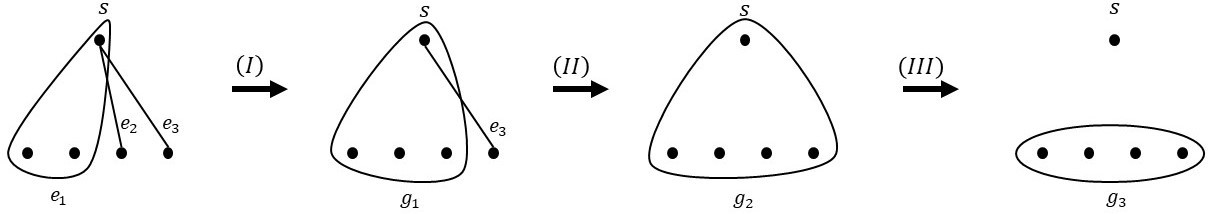
\includegraphics[width=\textwidth]{hypergraph-splitting-off-example-1.jpg}
\caption{Example of (local connectivity preserving) complete h-splitting-off at a vertex $s$ from a hypergraph. Consider the leftmost hypergraph where all hyperedge weights are one and the vertex $s$ is as labeled. Operations (I) and (II) correspond to h-merge almost-disjoint hyperedges operations and Operation (III) corresponds to an h-trim hyperedge operation.}
\label{figure:hypergraph-splitting-off-example-1}
\end{figure}

We will primarily be concerned with complete \emph{h-splitting-off} at a vertex from a \emph{hypergraph} and complete \emph{g-splitting-off} at a vertex from a \emph{graph}.  
Complete g-splitting-off at a vertex from a \emph{graph} is equivalent to the classical and well-studied notion of complete splitting-off at a vertex from a graph (for the definition of the classical notion in graphs, see \cite{Frank-book, nagamochi_ibaraki_2008_book}). 
We cast the results of Lov\'{a}sz \cite{Lov74, Lovasz-problems-book} and Mader \cite{Mad78} in the framework of our definitions now. Let $(G, w)$ be a \emph{graph} and let $s$ be a vertex in $G$. 
Lov\'{a}sz \cite{Lov74, Lovasz-problems-book} showed that if $d_{(G,w)}(\{s\})$ is even and $\min\{\lambda_{(G, w)}(u,v): u, v\in V\setminus \{s\}\}\ge K$ for some $K\ge 2$, then there exists a \emph{global} connectivity preserving complete g-splitting-off at the vertex $s$ from $(G, w)$. 
Mader \cite{Mad78} showed that if $d_{(G,w)}(\{s\})$ is even, there is no cut-edge\footnote{Equivalently, for every edge $e\in \delta_G(s)$ with $w(e)=1$, the removal of that edge does not disconnect the graph.} incident to $s$,  
%(i.e., for every hyperedge $e\in \delta(s)$ with $w(e)=1$, the removal of that hyperedge does not disconnect the hypergraph), 
and $(G, w)$ is connected, then there exists a \emph{local} connectivity preserving complete g-splitting-off at the vertex $s$ from $(G, w)$. 


We compare and contrast complete h-splitting-off at a vertex from a hypergraph and complete g-splitting-off at a vertex from a graph.  
Complete h-splitting-off at a vertex $s$ from a hypergraph enables the vertex $s$ to exit the hypergraph by informing its incident hyperedges about how to merge and trim themselves in  order to preserve degrees. In this sense, the definition of complete h-splitting-off at a vertex from a hypergraph serves the same role as complete g-splitting-off at a vertex from a graph. On the other hand, there are important differences between the two notions. Firstly, complete h-splitting-off at a vertex from a \emph{graph} may not necessarily be a graph (owing to the creation of hyperedges of size at least $3$) while it is an easy exercise to show that complete g-splitting-off at a vertex from a \emph{graph} will necessarily be a graph. %\kristof{Is this footnote needed?}\shubhang{I think we can remove it since it doesn't add value.}. 
%\footnote{Complete g-splitting-off at a vertex from a graph will necessarily be a graph: we leave this as an exercise for the reader.} 
Secondly, local/global connectivity preserving complete g-splitting-off at a vertex from a graph may not exist---see Figure \ref{figure:hypergraph-splitting-off-example-2}. 
%\footnote{Consider the graph $(G=(V, E), c: E\rightarrow \{1\})$, where $G$ is the $4$-vertex star graph with the vertex $s$ being the center of the star. Local connectivity preserving complete g-splitting-off at the vertex $s$ from $(G, c)$ does not exist.}. 

\begin{figure}[thb]
\centering
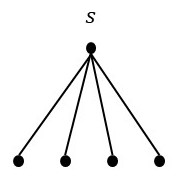
\includegraphics[scale=0.5]{hypergraph-splitting-off-example-2.jpg}
\caption{An example showing that global connectivity preserving complete g-splitting-off at a vertex from a graph may not exist. All edge weights are one and the vertex $s$ is as labeled.}
\label{figure:hypergraph-splitting-off-example-2}
\end{figure}

As our second main contribution, we show that local connectivity preserving complete h-splitting-off at a vertex from a hypergraph always exists and can be computed in strongly polynomial time (the rightmost hypergraph in Figure \ref{figure:hypergraph-splitting-off-example-1} is a local connectivity preserving complete h-splitting-off at the vertex $s$ from the hypergraph in Figure \ref{figure:hypergraph-splitting-off-example-2}). 

\begin{theorem}\label{thm:complete-splitting-off}
    Given a hypergraph $(G=(V, E), w_G: E\rightarrow \Z_+)$ and a vertex $s\in V$, there exists a strongly polynomial-time algorithm to find a local connectivity preserving complete h-splitting-off at $s$ from $(G, w_G)$. 
\end{theorem}
%The run-time of our algorithm is a somewhat large polynomial in the size of the input hypergraph. A crude upper bound on the run-time of our algorithm is $O(n^8m)$, where $n$ is the number of vertices and $m$ is the number of hyperedges in the input hypergraph. 

A distinction between Theorem \ref{thm:complete-splitting-off} and the graph splitting-off results of Lov\'{a}sz and Mader is that Theorem \ref{thm:complete-splitting-off} shows the existence of a local connectivity preserving complete h-splitting-off at a vertex from a hypergraph \emph{without any assumptions on the hypergraph} whereas Lov\'{a}sz's and Mader's results hold only under certain technical assumptions on the graph. In several applications of their results, additional arguments are needed to address cases where those technical assumptions do not hold. For this reason, we believe that Theorem \ref{thm:complete-splitting-off} could be useful in simplifying the arguments involved in some of the applications of Lov\'{a}sz's and Mader's graph splitting-off results (e.g., we will later see that the edge version of Menger's theorem in undirected \emph{graphs} follows in a straightforward fashion from Theorem \ref{thm:complete-splitting-off}). 
%In various applications of their results, satisfying these mild conditions requires additional technical arguments whereas . 

A crude run-time of our algorithm that proves Theorem \ref{thm:complete-splitting-off} is $O(|V|^6(|V|+|E|)^3)$.  %$O(|V|^8|E| + |V|^6|E|^3)$. 
%We leave the problem of finding efficient implementations of our algorithm as an intriguing open question. 
%(and it can be improved slightly using the recently discovered near-linear time max-flow algorithm). 
We understand that this run-time is impractical for applications. Nevertheless, we mention it here explicitly for the sake of completeness and as a potential starting point for future work: it would be interesting to design a near-linear time algorithm to find a local connectivity preserving complete h-splitting-off at a vertex from a weighted hypergraph.


\iffalse
\knote{Would be good to state the run-time.}
\shubhang{Crude runtime bound of the algorithm can be broken down as follows: Let $(H = (V, E),w:E\rightarrow\Z_+)$ and $p:2^V\rightarrow\Z$ be inputs to the algorithm. At the topmost level of recursion, we have that:
\begin{enumerate}
    \item $\functionMaximizationOracleStrongCover{p}((H,w), S, T , y)$ can be implemented in $O(|V|^2)$ \emph{max-flow} calls on hypergraphs with sizes linear in that of $(H,w)$. (Note: This is because for every pair of vertices $u,v \in {V\choose 2}$, we can implement $\lambda_{((G, c), (G_0, c_0), y_0)}(u, v)$ in the proof of \Cref{lemma:helper-for-p-max-oracle} using a single max-flow computation on hypergraph with $|V|+1$ vertices and $|E| + |V|$ hyperedges. Then, follow the proof of \Cref{lemma:helper-for-p-max-oracle} to see that having this oracle for every pair of vertices suffices). We will crudely upper-bound the max-flow query time as $O((|V|+|E|)|V||E|)$.
    %$O((|V||E|)^{1+o(1)})$ (randomized) time assuming polynomial edge weights. 
    (Note: the $|V||E|$ term in the runtime is a crude upper bound on the area of the hypergraph.)
    \item $\functionMaximizationOracle{p}((H,w), S, T, y)$ can be implemented using $O(|V|)$ queries to $\functionMaximizationOracleStrongCover{p}$ and $O(|V| + |E|)$ time per query (to construct the input). 
    \end{enumerate}
    
    Note that by \Cref{claim:WeakToStrong:p_i-oracle-using-p-oracle}, \functionMaximizationOracle{p_i} for every input function $p_i$ encountered during the recursion can be implemented using $O(|V|)$ queries to $\functionMaximizationOracleStrongCover{p}$ (recall $p$ is the input function to the algorithm). Thus,  if we bound the time required for all steps of the algorithm (except recursion) at just the topmost recursive level in terms of maximization-weak-oracle calls, then multiplying the bound by the recursion depth gives us a crude runtime bound on the overall algorithm. To get the bound we observe that
    \begin{enumerate}
    \item The family $\maximalTightSetFamily{p, H, w}$ can be computed in $O(|V|^2)$ queries to $\functionMaximizationOracle{p}$ by \Cref{lem:FunctionMaximizetionOracles:computing-maximal-pHw-tight-sets-with-p-max-oracle}. Each query takes $O(|V| + |E|)$ time (to construct the query input).
     This is also the time needed for step (4) of the algorithm (note that during the first recursive call we will need to compute the entire family).
    \item $\beta^M$ can be computed in $O(|V|^2)$ queries to $\functionMaximizationOracle{p}$. Each query takes $O(|V| + |E|)$ time (to construct the query input).
    \item $\beta^R$ can be computed in $1$ query to $\functionMaximizationOracle{p}$ in $O(|V| + |E|)$ time (to construct the query input).
    \item All other steps of the algorithm can be computed in $O(|V| + |E|)$ time per step. Since these steps are inconsequential from runtime perspective, we will ignore them in our runtime bound below.
\end{enumerate}
Thus, time bound per recursive call is (ignoring big-Oh notation for convenience)
\begin{align*}
    &[\text{time per  \functionMaximizationOracle{p} call}] \cdot [\text{$\#$ of  \functionMaximizationOracle{p} calls during rec. call}] &\\
    & = (|V| \cdot (|V| + |E| + [\text{time per  \functionMaximizationOracleStrongCover{p} call}])) \cdot |V|^2&\\
    &= (|V| \cdot (|V| + |E| + |V|^2\cdot[\text{time per max-flow call}])) \cdot |V|^2&\\
    &= (|V| \cdot (|V| + |E| + |V|^2\cdot(|V|+|E|)|V||E|)) \cdot |V|^2&\\
    & = (|V| + |E|)\cdot|V|^{6}|E|&
\end{align*}
Finally, we note that the recursion depth of our algorithm is $|E| + O(|V|)$ by \Cref{lem:WeakToStrongCover:NumberOfHyperedges}. Thus overall runtime of the algorithm is $O((|V| + |E|)^2\cdot|V|^{6}|E|)$ as remarked above.
}
\fi

%\shubhang{Assuming polynomially bounded hyperedge weights, the implementation of \functionMaximizationOracleStrongCover{p} can be improved to $\Tilde{O}(|V|)$ max flow computations by computing $|V|$ Gomory-Hu trees, each using $\Tilde{O}(1)$ max-flow computations via Abboud et. al.. Perhaps a single Gomory-Hu tree of a modified hypergraph suffices? If so, then we can compute the required Gomory-Hu tree (without needing the polynomially bounded hyperedge-weights assumption) using the classical $O(|V|)$ max-flows algorithm.}

\begin{remark}\label{remark:exp-sized-conn-preserving-splitting-off}
%\paragraph{An exponential-sized connectivity preserving complete h-splitting-off.} 
We note that existence of a local/global connectivity preserving complete h-splitting-off at a vertex from a hypergraph does not necessarily imply a polynomial-time algorithm to find it. 
This is because, 
%In fact, it is possible that 
a local/global connectivity preserving complete h-splitting-off at a vertex from a hypergraph $(G, w_G)$ could contain exponential number of hyperedges although $G$ contains only polynomial number of hyperedges. 
%, it does not necessarily imply that the number of hyperedges in $G^*$ is polynomial in the number of hyperedges in $G$. 
We give an example to illustrate this issue. 
Consider the graph $(G=(V, E), w_G)$ where $G$ is the star graph on $n+1$ vertices with $s$ being the center of the star and all edge weights are $2^{n-1}-1$. 
Consider the hypergraph $(H=(V, E_H), w_H)$ such that 
%$E_H$ contains every non-empty subset of $V\setminus\{s\}$ of size at least $2$ 
$E_H:=\{e: e\subseteq V\setminus \{s\} \text{ and } |e|\ge 2\}$ 
with all hyperedge weights being one. 
The hypergraph $(H, w_H)$ is a local connectivity preserving complete h-splitting-off at $s$ from $(G, w_G)$, but $(H, w_H)$ has exponential number of hyperedges although $(G, w_G)$ has only $n$ edges. 
%\knote{Is this example also showing that the Bernath-Kiraly algorithm could give an exponential-sized hypergraph?}
In order to design a polynomial-time algorithm to find a local connectivity preserving complete h-splitting-off at a vertex from a hypergraph, a necessary step is to show the existence of a local connectivity preserving complete h-splitting-off at a vertex from a hypergraph that contains only polynomially many \emph{additional} hyperedges. 
For the star graph $(G,w_G)$ with edge weights $2^{n-1}-1$ mentioned above, the hypergraph $(H'=(V, E_{H'}), w_{H'})$ containing only one hyperedge, namely $E_{H'}:=\{V\setminus \{s\}\}$ with the weight of that hyperedge being $2^{n-1}-1$ is also a local connectivity preserving complete h-splitting-off at $s$ from $(G,w_G)$. 
One of the features of our algorithmic proof of Theorem \ref{thm:complete-splitting-off} is the existence of a local connectivity preserving complete h-splitting-off at a vertex from a hypergraph that contains only polynomially many additional hyperedges. 
%\knote{Say a bit about why existence does not necessarily imply an efficient algorithm to find it---expecially in the weighted case. Would be good to have an example of a weighted hypergraph with polynomial number of hyperedges, but a bad choice of sequence of splitting-off operations leads to an exponential number of hyperedges.}
\end{remark}

As our third main contribution, 
we present two applications of Theorem \ref{thm:complete-splitting-off}. 
%illustrate the usefulness of Theorem \ref{thm:complete-splitting-off} by presenting two applications. 

\paragraph{Application 1: Constructive characterization of $k$-hyperedge-connected hypergraphs.}
For the purposes of this application, 
graphs and hypergraphs will refer to multi-graphs and multi-hypergraphs, respectively.
%we will consider multi-hypergraphs and multi-graphs. 
Let $k$ be a positive integer. A graph $G=(V, E)$ is \emph{$k$-edge-connected} if $d_{G}(X)\ge k$ for every non-empty proper subset $X\subsetneq V$. 
Constructive characterization of $k$-edge-connected graphs is a central problem in graph theory. 
It is well-known that a graph is $1$-edge-connected if and only if it admits a spanning tree. 
Robbins' \cite{Rob39} showed that a graph is $2$-edge-connected if and only if it admits an ear decomposition (see \cite{Frank-book} for definition of ear decomposition). 
Generalizing Robbins' result, 
Lov\'{a}sz \cite{Lov74, Lovasz-problems-book} gave a constructive characterization of $k$-edge-connected graphs for \emph{even} $k$ using his result on global connectivity preserving complete g-splitting-off at a vertex from a graph. 
%An application of this characterization is an alternate proof of Nash-Williams' weak orientation theorem \cite{??} \knote{Do we have a citation for this?}. 
Mader \cite{Mad78} gave a constructive characterization of $k$-edge-connected graphs for \emph{odd} $k$ using his result on local connectivity preserving complete g-splitting-off at a vertex from a graph. 
Motivated by these results, we present a constructive characterization of $k$-hyperedge-connected hypergraphs using our splitting-off result in Theorem \ref{thm:complete-splitting-off}.
A hypergraph $G=(V, E)$ is defined to be \emph{$k$-hyperedge-connected} if $d_{G}(X)\ge k$ for every non-empty proper subset $X\subsetneq V$. 


Both Lov\'{a}sz's and Mader's constructive characterizations of $k$-edge-connected graphs are based on a pinching operation in graphs. Our constructive characterization of $k$-hyperedge-connected hypergraphs is also based on a pinching operation, but our pinching operation is defined for hypergraphs. We define this operation now (see \Cref{fig:hypergraph-pinching-example} for an example). %\knote{Include a figure to explain the pinching operation.}

\begin{definition}\label{def:pinching-operation}
    Let $G = (V, E)$ be a hypergraph and $p,k \in \Z_+$ be positive integers such that $p \leq k$. In \emph{$(k, p)$-pinching} hyperedges of $G$, we obtain a new hypergraph by performing the following sequence of operations:
    \begin{enumerate}
        \item pick $p$ distinct hyperedges $e_1, \ldots, e_p \in E$,
        \item pick $p$ positive integers $t_1, \ldots, t_p \in \Z_+$ such that $\sum_{i=1}^p t_i = k$,
        \item for each $i \in [p]$, choose a partition of the hyperedge $e_i$ into $t_i$ non-empty parts $e_i = \uplus_{j \in [t_i]} f_i^j$,
        \item remove the hyperedges $e_1, \ldots, e_p$ from the hypergraph $G$,
        \item add a new vertex $s$ and hyperedges $\{f_i^j \cup \{s\} : j \in [t_i], i \in [p]\}$ to the hypergraph $G$.
    \end{enumerate}
\end{definition}

%\shubhang{We note that the pinching operation is the \emph{inverse} of the h-splitting-off operation.}\knote{This might be too much detail for the reader to verify here. So, better not to state it here.} 
\begin{figure}[thb]
    \centering
    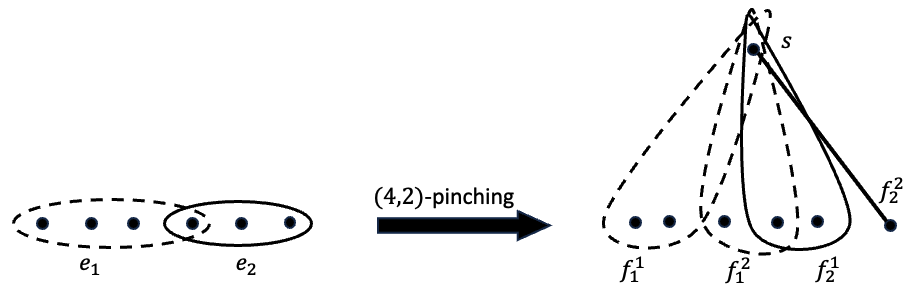
\includegraphics[width=0.7\textwidth]{hypergraph_pinching_example.png}
    \caption{An example of a $(4,2)$-pinching operation. Here, $t_1 = t_2 = 2$.}
    \label{fig:hypergraph-pinching-example}
\end{figure}
%\knote{Remove $H$ and the box from Figure \ref{fig:hypergraph-pinching-example}.}
With this definition of pinching, we show the following constructive characterization of $k$-hyperedge-connected hypergraphs. 
\begin{restatable}{theorem}{thmConstructiveCharacterization}\label{thm:k-EC-hypergraph-characterization}
    Let $k \in \Z_+$ be a positive integer. A hypergraph $G = (V, E)$ is $k$-hyperedge-connected if and only if $G$ can be obtained by starting from the single vertex hypergraph with no hyperedges and repeatedly applying one of the following two operations:
    \begin{enumerate}
        \item add a new hyperedge over a subset of vertices of the existing hypergraph, and
        \item $(k, p)$-pinching hyperedges of the existing hypergraph for some positive integer $p \leq k$.
    \end{enumerate}
\end{restatable}
Our proof of Theorem \ref{thm:k-EC-hypergraph-characterization} is constructive: i.e., given a $k$-hyperedge-connected hypergraph $G$, our proof gives a polynomial-time algorithm to construct a sequence of hypergraphs $G_0, G_1, G_2, \ldots, G_t$, where $G_0$ is the single vertex hypergraph with no hyperedges, $G_t=G$ and for each $i\in [t]$, the hypergraph $G_i$ is obtained from $G_{i-1}$ by either adding a new hyperedge over a subset of vertices in $G_{i-1}$ or by $(k,p)$-pinching hyperedges in $G_{i-1}$ for some positive integer $p\le k$. 

\begin{remark}
Robbins' constructive characterization of $2$-edge-connected graphs and Lov\'{a}sz's constructive characterization of $2k$-edge-connected graphs find applications in graph orientation problems---e.g., 
%Robbins' result implies that a graph has a strongly connected orientation if and only if it is $2$-edge-connected if and only if it has a strongly connected orientation and
%Lov\'{a}sz's result implies that a graph has a strongly $k$-arc-connected orientation if and only if it is $2k$-edge-connected. 
Robbins' result leads to an algorithm to find a strongly connected orientation of $2$-edge-connected graphs and 
Lov\'{a}sz's result leads to an algorithm to find a strongly $k$-arc-connected orientation of $2k$-edge-connected graphs. In fact, the latter leads to an alternative proof of Nash-Williams' \emph{weak orientation theorem} \cite{NW60}. 
%Alternative proof is here: https://math.mit.edu/~goemans/18438F09/lec17.pdf
%There is no known generalization of Nash-Williams' weak orientation theorem to hypergraphs. Our above characterization might be a helpful tool towards identifying possible generalizations to hypergraphs.
Along the same vein, we hope that our above characterization of $k$-edge-connected hypergraphs might find applications in hypergraph orientation problems. 
\end{remark}


\paragraph{Application 2.1: Steiner Rooted $k$-arc-connected Orientation of Graphs.}
Orienting a graph to achieve high connectivity is a fundamental area in graph theory, combinatorial optimization, and algorithms. Let $G=(V, E)$ be an undirected graph.  An \emph{orientation} $\overrightarrow{G}$ of $G$ is a directed graph obtained by assigning a direction to each edge of $G$. 
Let $G=(V, E)$ be an undirected graph, $T\subseteq V$ be a set of terminals, $r\in T$ be a root vertex, and $k$ be a positive integer. 
%In rooted Steiner $k$-arc-connected orientation of graphs, we are given an undirected graph $G=(V, E)$, a subset $T\subseteq V$ of terminals, a root vertex $r\in T$, and a positive integer $k$. 
An orientation $\overrightarrow{G}$ of $G$ is defined to be \emph{Steiner rooted $k$-arc-connected} if there exist $k$ arc-disjoint paths in $\overrightarrow{G}$ %from $r$ to $t$ 
from $t$ to $r$ 
for every terminal $t\in T\setminus \{r\}$. 
In \textsc{Max Steiner Rooted-Connected Orientation} problem, the goal is to find the maximum integer $k$ and an orientation $\overrightarrow{G}$ of $G$ such that $\overrightarrow{G}$ is Steiner rooted $k$-arc-connected. 
\textsc{Max Steiner Rooted-Connected Orientation} generalizes two classic problems in graph theory: The case of $|T|=2$ is the max edge-disjoint $\{r,v\}$-paths problem and is solved via Menger's theorem. The case of $T=V$ is the max edge-disjoint spanning trees problem and is solved via Tutte and Nash-Williams' theorem \cite{Tu61, NW61}. We mention that both these problems are also generalized by the Steiner Tree Packing problem and the associated Kriesell's conjecture \cite{Kri03, JMS03, Lau07}, but we will not focus on that generalization. 

Kir\'{a}ly and Lau \cite{Kiraly-Lau} introduced the \textsc{Max Steiner Rooted-Connected Orientation}, showed that it is NP-hard, and gave a $2$-approximation via an approximate min-max relation. We state their approximate min-max relation now. 
An undirected graph $G$ is \emph{Steiner $k$-edge-connected} if $\lambda_G(u,v)\ge k$ 
%there exist $k$ edge-disjoint paths between 
for every pair of distinct terminals $u, v\in T$. 
It is clear that if the graph $G$ has a Steiner rooted $k$-arc-connected orientation, then $G$ should be Steiner $k$-edge-connected. However, the converse is not necessarily true. Kir\'{a}ly and Lau observed that if the graph is Steiner $2k$-edge-connected, then it has a Steiner rooted $k$-arc-connected orientation. 

\begin{theorem}[Kir\'{a}ly and Lau \cite{Kiraly-Lau}]\label{thm:rooted-steiner-orientation-in-graphs}
Let $G=(V, E)$ be an undirected graph, $T\subseteq V$ be a subset of terminals, $r\in T$ be the root vertex, and $k$ be a positive integer. If $G$ is Steiner $2k$-edge-connected, then it has a Steiner rooted $k$-arc-connected orientation. 
\end{theorem}

Kir\'{a}ly and Lau observed that Theorem \ref{thm:rooted-steiner-orientation-in-graphs} follows immediately from Nash-Williams' \emph{strong orientation} theorem. 
Nash-Williams' \emph{strong orientation} theorem \cite{NW60} states that every undirected graph $G=(V, E)$ admits an orientation $\overrightarrow{G}$ such that $\lambda_{\overrightarrow{G}}(u,v)\ge \lfloor \lambda_G(u,v)/2\rfloor$ for every distinct $u, v\in V$, where $\lambda_{\overrightarrow{G}}(u,v)$ is the maximum number of arc-disjoint directed paths from $u$ to $v$ in $\overrightarrow{G}$. 
In this work, we give an alternative proof of Theorem \ref{thm:rooted-steiner-orientation-in-graphs} that does not rely on Nash-Williams' strong orientation theorem. Instead, we use Theorem \ref{thm:complete-splitting-off}. 
Our proof strategy is unique since it proves an orientation result for \emph{graphs} using tools developed for \emph{hypergraphs}. 

\begin{remark}
Nash-Williams' proof of the strong orientation theorem \cite{NW60} is a sophisticated inductive argument. Giving a simple and more insightful proof of the strong orientation theorem has been a central topic of interest in graph theory and combinatorial optimization (see \cite{Frank93:Applications-of-submod-functions}). Mader \cite{Mad78} gave a different proof of the strong orientation theorem using his local connectivity preserving splitting-off theorem, but his proof also involved sophisticated technical arguments. Frank \cite{Frank93:Applications-of-submod-functions} condensed the ideas of both Nash-Williams and Mader to present a proof of the strong orientation theorem using Mader's local connectivity preserving splitting-off, but it is still technically complicated. The technical complication in using Mader's local connectivity preserving splitting-off result arises from the assumptions that need to be satisfied by the vertex to be split-off. In contrast, our splitting-off result for hypergraphs (namely, Theorem \ref{thm:complete-splitting-off}) does not need any assumptions on the vertex to be split-off. In light of these considerations, our proof of Theorem \ref{thm:rooted-steiner-orientation-in-graphs} using Theorem \ref{thm:complete-splitting-off} provides hope that Theorem \ref{thm:complete-splitting-off} (or the ideas therein) could be used to give a conceptually simpler proof of Nash-Williams' strong orientation theorem. 
\end{remark}


\paragraph{Application 2.2: Steiner Rooted $k$-hyperarc-connected Orientation of Hypergraphs.}
Orienting \emph{hypergraphs} is also a fundamental area in graph theory and combinatorial optimization (see Frank's book \cite{Frank-book}) 
%. We note that fundamental results in hypergraph orientation have recently been used in coding theory \cite{AGL23}.
with far reaching implications. For example, Woodall's conjecture can be reformulated as a hypergraph orientation problem \cite{egres-open-problem-on-head-disjoint-sco}; moreover,  
hypergraph orientation results have recently been used in coding theory \cite{AGL23}.
%work in coding theory \cite{AGL23} that has exploited hypergraph orientation results). 
%the classic Woodall's conjecture can be phrased as a hypergraph orientation problem. 
Kir\'{a}ly and Lau \cite{Kiraly-Lau} showed that the approximate min-max relation in Theorem \ref{thm:rooted-steiner-orientation-in-graphs} also holds for hypergraphs. To state their result, we need some terminology in hypergraph orientations. 

Let $G=(V, E)$ be a hypergraph. An \emph{orientation} $\overrightarrow{G}=(V, E, \head:E\rightarrow V)$ of $G$ is a directed hypergraph obtained by assigning a unique head vertex $\head(e)\in e$ for each $e\in E$. 
%and setting $\tails(e):=e\setminus \head(e)$ for each $e\in E$. 
A pair $(e, \head(e))$ is denoted as a \emph{hyperarc} with the head of the hyperarc being $\head(e)$ and the tails of the hyperarc being $e\setminus \head(e)$. 
%A hyperarc is a hyperedge with a designated head vertex and other vertices as tail vertices. 
Let $G=(V, E)$ be a hypergraph, $T\subseteq V$ be a set of terminals, $r\in T$ be a root vertex, and $k$ be a positive integer. An orientation $\overrightarrow{G}$ of $G$ is defined to be \emph{Steiner rooted $k$-hyperarc-connected} if there exist $k$ hyperarc-disjoint paths in $\overrightarrow{G}$ 
%from $r$ to $t$ 
from $t$ to $r$ 
for every terminal $t\in T\setminus \{r\}$. Here, a path from $t$ to $r$ in a directed hypergraph is an alternating sequence of distinct vertices and hyperarcs $t=v_1, a_1, v_2, a_2, ..., a_{\ell-1}, v_{\ell}=r$ such that 
%$v_i$ is the head of $a_i$ and $v_{i+1}$ is a tail of $a_i$ \knote{Definition needs to be adjusted to go with convention.} 
$v_i$ is a tail of $a_i$ and $v_{i+1}$ is the head of $a_i$ 
for every $i\in [\ell-1]$. We say that a hypergraph $G$ is \emph{Steiner $k$-hyperedge-connected} if 
%there exist $k$ hyperedge-disjoint paths between 
$\lambda_G(u,v)\ge k$ for 
every pair of distinct terminals $u, v\in T$. 
%Here, a path in a hypergraph is an alternative sequence of distinct vertices and hyperedges $v_1, e_1, v_2, e_2, ..., e_{\ell-1}, v_{\ell}$ such that $v_i, v_{i+1}\in e_i$ for every $i\in [\ell-1]$. 
It is clear that if the hypergraph $G$ has a Steiner rooted $k$-hyperarc-connected orientation, then $G$ should be Steiner $k$-hyperedge-connected. However, the converse is not necessarily true. Kir\'{a}ly and Lau \cite{Kiraly-Lau} showed that if the hypergraph is Steiner $2k$-hyperedge-connected, then it has a Steiner rooted $k$-hyperarc-connected orientation. 

\begin{restatable}[Kir\'{a}ly and Lau \cite{Kiraly-Lau}]{theorem}{thmRootedSteinerArcConnectedOrientationsHypergraphs}\label{thm:rooted-steiner-orientation-in-hypergraphs}
Let $G=(V, E)$ be a hypergraph, $T\subseteq V$ be a subset of terminals, $r\in T$ be the root vertex, and $k$ be a positive integer. If $G$ is Steiner $2k$-hyperedge-connected, then it has a Steiner rooted $k$-hyperarc-connected orientation. 
\end{restatable}
Kir\'{a}ly and Lau's proof of Theorem \ref{thm:rooted-steiner-orientation-in-hypergraphs} was based on careful uncrossing and contractions. In this work, we give an alternative proof of Theorem \ref{thm:rooted-steiner-orientation-in-hypergraphs} using Theorem \ref{thm:complete-splitting-off}. 
%Our proof reveals the source of the $2$ factor in the min-max relation, namely, it is the gap between connectivity and weak-partition-connectivity of hypergraphs (see Definition \ref{defn:weak-partition-connectivity} for the definition of weak-partition-connectivity). 
Our proof of \Cref{thm:rooted-steiner-orientation-in-hypergraphs} reveals the source of the $2$-factor gap in the approximate min-max relation of Kir\'{a}ly and Lau for \textsc{Max Steiner Rooted-Connected Orientation Problem}: it arises from the $2$-factor gap between connectivity and weak-partition-connectivity of hypergraphs (see Definition \ref{defn:weak-partition-connectivity} for the definition of weak-partition-connectivity and Lemma \ref{lem:2k-conn-implies-k-weak-pc}). 

\iffalse
\knote{
\begin{remark}
As mentioned earlier, Theorem \ref{thm:rooted-steiner-orientation-in-graphs} follows immediately from Nash-Williams' strong orientation theorem for graphs. In a similar vein, one would hope that a generalization of Nash-Williams' strong orientation theorem for hypergraphs might help prove Theorem \ref{thm:rooted-steiner-orientation-in-hypergraphs}. However, there is no known generalization of Nash-Williams' strong orientation theorem for hypergraphs (also see Remark \ref{??}). We hope that 
\end{remark}
}
\fi

\begin{remark}
Our proof technique for Theorems \ref{thm:rooted-steiner-orientation-in-graphs} and \ref{thm:rooted-steiner-orientation-in-hypergraphs} using Theorem \ref{thm:complete-splitting-off}---i.e., via the local-connectivity preserving splitting-off operation in hypergraphs---also leads to an alternate proof of Menger's theorem in \emph{undirected} graphs and hypergraphs (edge-disjoint version). For details, we refer the reader to Section \ref{sec:rooted-steiner-connected-orientations} where we discuss a proof of Menger's theorem using \Cref{thm:complete-splitting-off} as a warm-up towards a proof of Theorems \ref{thm:rooted-steiner-orientation-in-graphs} and \ref{thm:rooted-steiner-orientation-in-hypergraphs}. 
\end{remark}

Both Theorems \ref{thm:rooted-steiner-orientation-in-graphs} and \ref{thm:rooted-steiner-orientation-in-hypergraphs} can be extended to weighted graphs/hypergraphs (by considering parallel copies of edges/hyperedges). The weighted version of Theorems \ref{thm:rooted-steiner-orientation-in-graphs} and \ref{thm:rooted-steiner-orientation-in-hypergraphs} can also be shown to admit strongly polynomial-time algorithms using our proof strategy as well as the proof strategy of Kir\'{a}ly and Lau. We avoid stating the weighted versions in the interests of brevity. 


%\knote{Might be good to discuss only the graph version of the result here instead of the hypergraph version. Graph orientations involve far less notation than hypergraph orientations. Readers might follow graph orientations better than hypergraph orientations and might appreciate the flavor of the proof. We can mention the more general result for hypergraph orientations at the end.}

